\documentclass{article}
\usepackage{graphicx}
\usepackage{caption}
\usepackage{subcaption}

\begin{document}

\title{Experiment Report: \texttt{\{experiment\}}}
\author{Automated experiment report}
\date{\today}

\maketitle

\section{Introduction}
This document presents the results for my experiment \texttt{\{experiment\}}. Below are the key figures generated during the analysis.

\section{Figures}
Figure \ref{fig:Fig2_B} shows the number of positive co-occurrences that were determined for all treatements. We also show the numbers of matches these co-occurrences had with either interactions (orange) and/or environmental preference similarity (green). 

\begin{figure}[h!]
\centering
  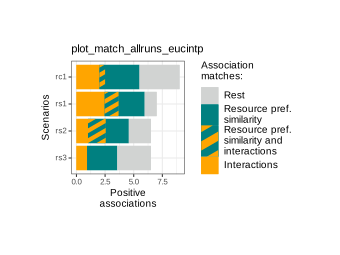
\includegraphics[width=1\linewidth]{figures/Fig2_B.svg}
  \caption{}
  \label{fig:Fig2_B}
\end{figure}

Figure \ref{fig:Fig2_B} shows the number of negative co-occurrences and corresponding matches.

\begin{figure}[h!]
\centering
  \includegraphics[width=1\linewidth]{figures/correlations_withinC.svg}
  \caption{}
  \label{fig:correlations_withinC}
\end{figure}

Bye!

\end{document}

